% !TEX root = ../main.tex
%
\chapter{Related Work}
\label{sec:related}

\section{Nerfstudio}
\label{sec:related:nerfstudio}

NeRFStudio \cite{tancik_nerfstudio_2023} represents a significant advancement in making Neural Radiance Fields accessible to non-technical users. Its design focuses on modularity, ease of use, and integration capabilities, which are crucial for practical applications and academic research.

\paragraph{Modularity}
NeRFStudio is built on a modular framework that allows users to easily customize and extend their NeRF implementations. This modularity supports various input data formats, making it versatile for different real-world scenarios.

\paragraph{Real-Time Web Viewer}
One of the standout features of NeRFStudio is its real-time web viewer, which enables visualization of NeRF training and outputs directly through a web browser. This eliminates the need for high-end local GPU setups, broadening the tool's accessibility \cite{noauthor_nerfstudio-projectviser_2024}.

\begin{figure}[h!]
  \centering
  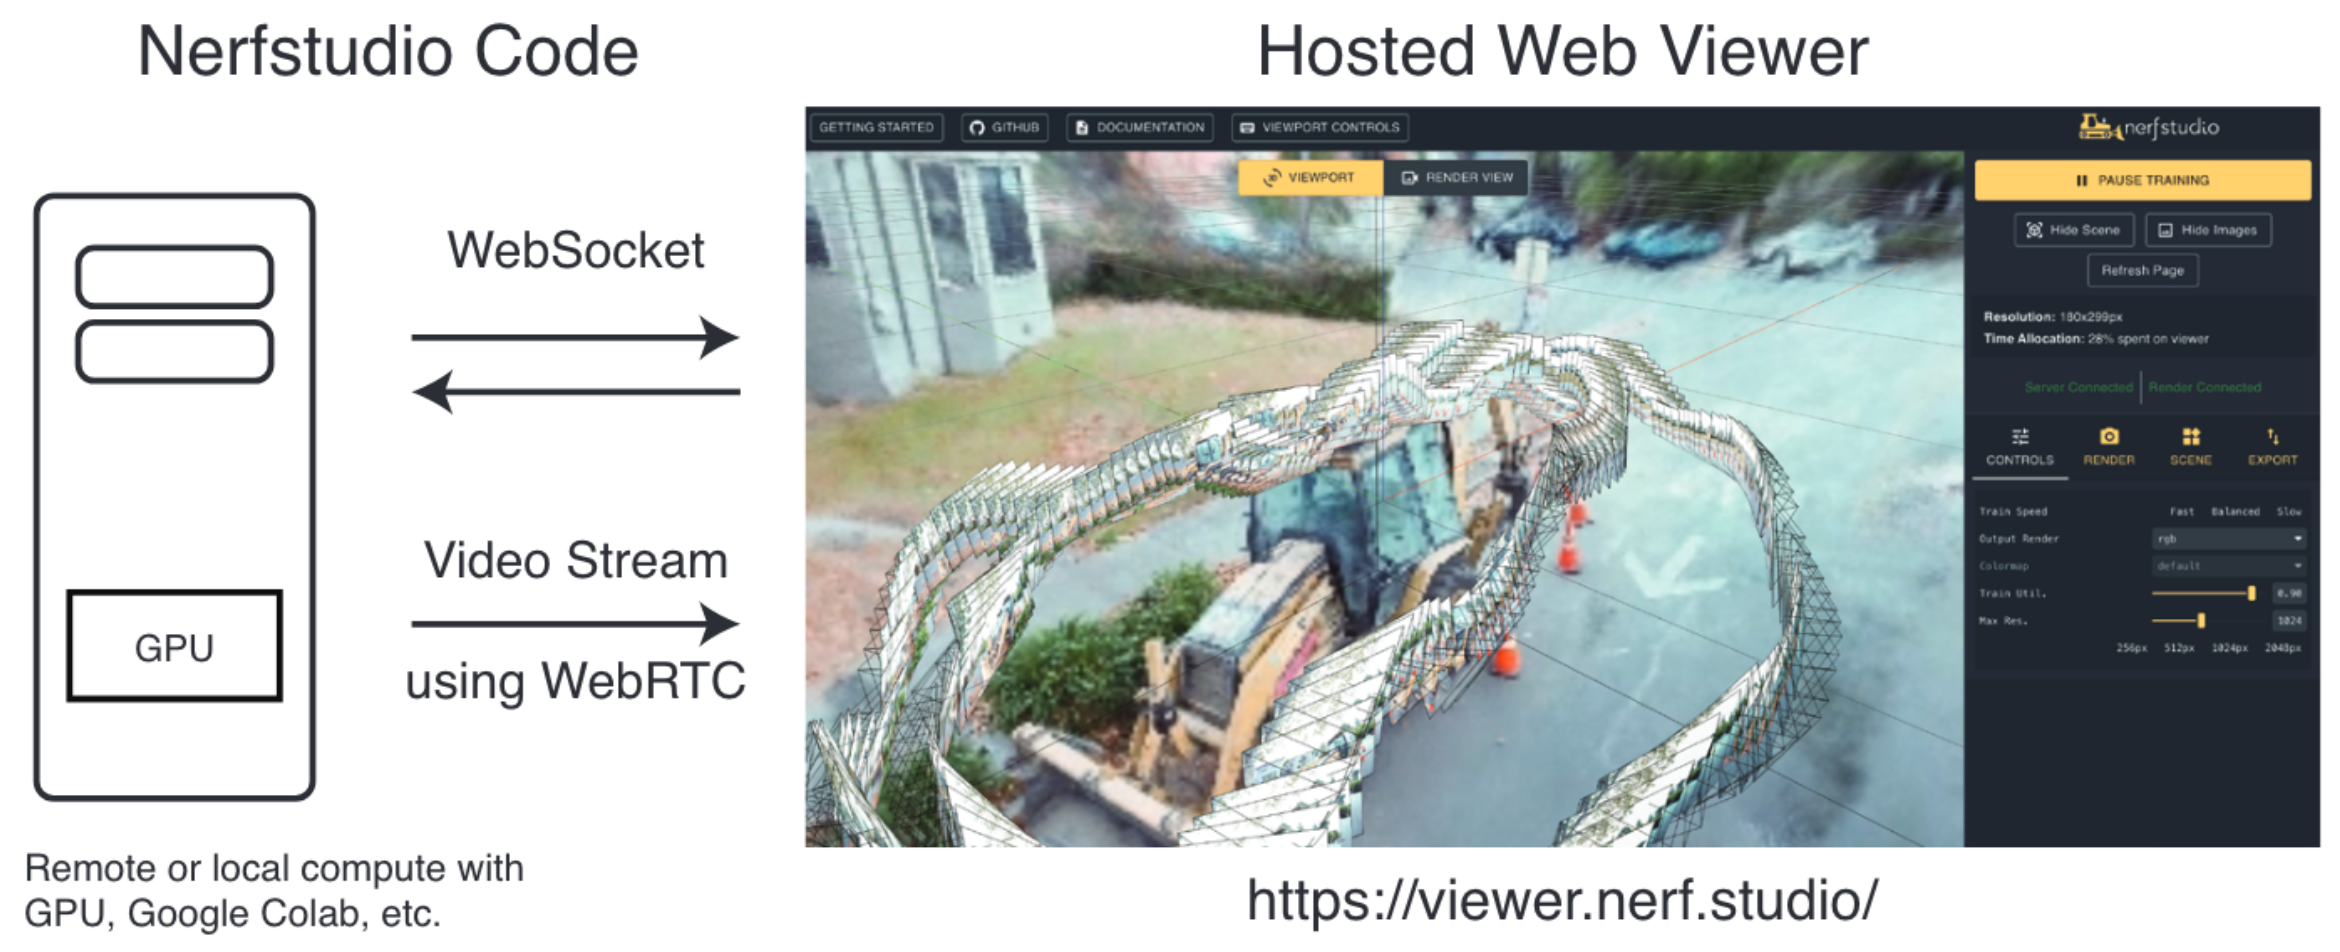
\includegraphics[width=0.7\textwidth]{figures/related-nerfstudio-viewer.png}
  \caption{NeRFStudio's real-time web viewer. (from \cite{tancik_nerfstudio_2023})}
  \label{fig:nerfstudio-viewer}
\end{figure}

\paragraph{Flexibility of Data Handling}
NeRFStudio simplifies the process of importing and exporting data, supporting a wide range of formats to enhance usability. Users can easily import images and videos, including data from mobile capture apps such as Polycam \cite{noauthor_polycam_nodate} and Record3D \cite{noauthor_record3d_nodate}. Additionally, the framework supports exporting results in various formats such as videos, point clouds, and meshes. This flexibility allows users to seamlessly integrate NeRF outputs into diverse applications across visual effects, gaming, and digital arts, catering to a broad spectrum of creative and technical needs.

\paragraph{Community and Open-Source Contribution}
Being open-source, NeRFStudio encourages community-driven development and continuous improvement, facilitating updates that keep pace with the latest research and technological advances. This openness also allows users to adapt the tool to their specific needs.

\paragraph{Shortcomings and Areas for Improvement}

Despite advancements, NeRFStudio's technical complexity and reliance on command-line interfaces for key operations like model training and data preprocessing remain significant barriers. These aspects limit its accessibility to those with specific technical skills and deter broader creative uses. The user experience still requires technical knowledge, underscoring the need for more intuitive interfaces that simplify interaction and expand its user base beyond technical specialists.

\section{Luma AI}
\label{sec:related:lmua}

\section{Photogrammetry}
\label{sec:related:photogrammetry}
